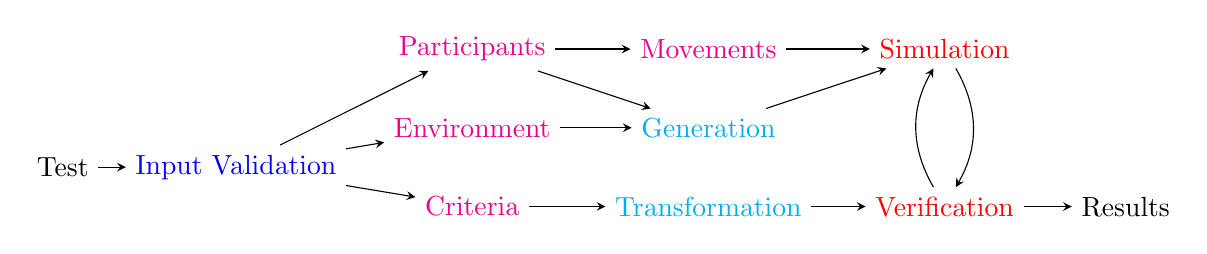
\begin{tikzpicture}[%
        ->,
        >=stealth
    ]
    \node at (-3.2,0) (Tester) {Test};
    \node at (-1,0) (Validation) {\textcolor{blue}{Input Validation}};
    \node at (2,0.5) (Environment) {\textcolor{magenta}{Environment}};
    \node at (2,1.5) (Participants) {\textcolor{magenta}{Participants}};
    \node at (5,1.5) (Movements) {\textcolor{magenta}{Movements}};
    \node at (2,-0.5) (Criteria) {\textcolor{magenta}{Criteria}};
    \node at (5,-0.5) (Transform) {\textcolor{cyan}{Transformation}};
    \node at (5,0.5) (Generation) {\textcolor{cyan}{Generation}};
    \node at (8,1.5) (Simulation) {\textcolor{red}{Simulation}};
    \node at (8,-0.5) (Verification) {\textcolor{red}{Verification}};
    \node at (10.3,-0.5) (Results) {Results};
    \path
        (Tester) edge (Validation)
        (Validation) edge (Environment)
        (Environment) edge (Generation)
        (Generation) edge (Simulation)
        (Validation) edge (Participants)
        (Participants) edge (Movements)
        (Movements) edge (Simulation)
        (Participants) edge (Generation)
        (Validation) edge (Criteria)
        (Criteria) edge (Transform)
        (Transform) edge (Verification)
        (Verification) edge[bend left] (Simulation)
        (Simulation) edge[bend left] (Verification)
        (Verification) edge (Results);
\end{tikzpicture}
